\documentclass[12pt]{memoir}

\usepackage{titling}

% Figures and controlling packages
\usepackage{float}
\usepackage{wrapfig}

% logo for the title page
\usepackage{adjustbox}
\newcommand{\swlogo}{
  \adjustbox{valign=t}{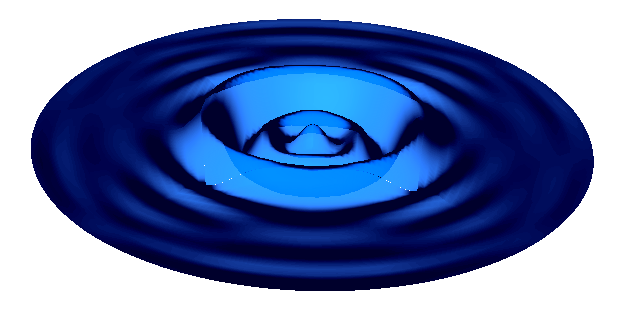
\includegraphics[width=0.25\textwidth]{images/shallowWater.png}}
}


% Adjusting the section,chapter, etc. headings
\usepackage{titlesec}
\newcommand*{\justifyheading}{\raggedleft}

\titleformat{\chapter}[display]
  {\normalfont\sffamily\huge\bfseries\justifyheading\color{blue}}
  {\chaptertitlename\ \thechapter}{20pt}{\Huge}
\titleformat{\section}
  {\normalfont\sffamily\Large\bfseries\color{cyan}}
  {\thesection}{1em}{}

\usepackage[margin=1.0in]{geometry}
\usepackage{amsmath,amsthm}
%\usepackage{breqn}
\usepackage{amsfonts}
\usepackage{amssymb}
\usepackage[mathscr]{euscript}
\usepackage{graphicx}
\usepackage{verbatim}
\usepackage[round]{natbib}
\usepackage{appendix}
\usepackage{xcolor}


% Header and Footer
\makeevenhead{myheadings}{}{}{}
\makeoddhead{myheadings}{}{}{}{}

\makeevenfoot{myheadings}{ {\fontfamily{cmss}\selectfont \theauthor} }{{\fontfamily{cmss}\selectfont schoonover.numerics@gmail.com }}{\thepage}

\makeoddfoot{myheadings}{ {\fontfamily{cmss}\selectfont \theauthor  } }{{\fontfamily{cmss}\selectfont schoonover.numerics@gmail.com} }{\thepage}

\makefootrule{myheadings}{\textwidth}{\normalrulethickness}{0ex}

\author{Joe Schoonover}
\title{Discontinuous Galerkin}
\date{}




\begin{document}
\frontmatter
% Doing a custom title-page
\begin{titlingpage}
    
        \vspace*{2cm}

   % Setup up the main and sub-titles with the logo
   {\fontfamily{cmss}\selectfont
     \begin{tabular}{l r}
           & \HUGE{\textbf{ \thetitle }}\\
           & \HUGE{\textbf{ Spectral Element Method }}\\
   \swlogo & \\
           & \huge{\textbf{\textcolor{blue}{Shallow Water Equations}}}
        \end{tabular}
    }    
 
        \vspace{1cm}
        

         
        \vspace{2cm}
        
     \begin{center}
     
        %Do a subtitle here if you like
        {\fontfamily{cmss}\selectfont
        \huge{
           Software Documentation
        }
        
        \vspace{1.5cm}
        
        % Enter the author's name
        \textbf{
        \large{
           \theauthor 
         }}}
        
        \vfill
        
        
     \end{center}
        
    
\end{titlingpage}


{\fontfamily{cmss}\selectfont
\tableofcontents
}
\mainmatter

% Special Style
\pagestyle{myheadings}

\chapter{Overview and Motivation}

\chapter{QuickStart}
At this point, you have probably unpacked the \texttt{SEM} software libraries in your favorite directory. Here, this will be denoted with ``\texttt{install/dir}.'' This part of the documentation will walk you through the compilation and execution procedures for an instance of the \texttt{DGSEM\_ShallowWater\_Class}. Additionally, steps will be shown for modifying the initial conditions and the mesh to demonstrate the ability to modify the problem. More advanced modifications are discussed in Chapter \ref{chap:Class}. \\

Overall, there are three main steps to performing a simulation
\begin{enumerate}
\item Generate a mesh.
\item Generate initial conditions.
\item Integrate in time.
\end{enumerate}

The first step is achieved by using the SpecMesh software. This generates a mesh from boundary and internal curve inputs in the ``ISM-v2'' format (see the SpecMesh documentation for details on this). Initial conditions are generated using a driver program \texttt{ShallowWater\_Init.f90}. This driver reads in the mesh file output from SpecMesh, computes initial conditions specified by the user within the program, and writes an initial pickup file. Finally, the main driver \texttt{ShallowWater\_Main.f90} reads the mesh and pickup file and performs integration forward in time, manages diagnostic calculations, and file I/O.\\

We will begin by working with the ``gravity-wave'' example. Once you are within the installation directories, you should see the subdirectories
\begin{verbatim}
doc/  examples/  src/  testing/
\end{verbatim}
Change directories into \texttt{examples/} and into the subdirectory \texttt{shallowwater}.
\begin{verbatim}
cd examples/shallowwater
\end{verbatim}
As more validated experiments are conducted with the shallow-water solver, more examples will be found here. For now, we will go into the \texttt{gravity-wave} directory, underneath which you will find the subdirectories
\begin{verbatim}
build/   init/  meshgen/  run/
\end{verbatim}
In the first step, we will modify the make file to ensure we are using the correct compiler and all SEM source directory is set appropriately. The makefile is located in the \texttt{build} directory. Change directories into the \texttt{build} directory and open up the makefile in your favorite text editor. You should see something like 
\begin{verbatim}
# Specify the SEM source code directory
SRCDIR=/home/joe/Desktop/work/SEM/SEM_v2.0/src/
FC=gfortran

# Additional library and includes directories
LIB=
INC= 

# Fortran compilation flags
FFLAGS=-O3 -fopenmp
\end{verbatim}
Set the \texttt{SRCDIR} to the directory where you installed the SEM libraries and include \texttt{src/} at the end (similar to what is shown). Ensure  that the fortran compiler is set appropriately in the variable \texttt{FC}. Lastly, any optimization, debugging, or warning compilation flags should be set under \texttt{FFLAGS}.\\


Now you are ready to compile. There are three commands available with this makefile.
\begin{enumerate}
\item \texttt{make Initialize}
\item \texttt{make ShallowWater}
\item \texttt{make clean}
\end{enumerate}
We will build the initial condition generator and the main driver by using the first two commands. Copy the executables into the run directory and clean up your build directory (if you like)
\begin{verbatim}
make Initialize
make ShallowWater
cp Initialize ShallowWater ../run/
make clean
\end{verbatim}
Compilation is done at this point.\\

Now, we proceed to make the mesh. At this point you should have compiled SpecMesh and moved the executable into the \texttt{meshgen/} folder. Currently, two control files have been placed in the \texttt{meshgen/} directory for this experiment; they are \texttt{square.control} and \texttt{circle.control}. Pick your favorite, and run SpecMesh with that control file. Copy the .mesh file into the run directory. For example,
\begin{verbatim}
./SpecMesh+3D < circle.control
cp circle.mesh ../run/
\end{verbatim}
Mesh generation is now complete.\\

Change directories into the run directory. Running the code is as simple as running the initial condition generator and running the main driver. Verify that the file \texttt{runtime.params} specifies the correct \texttt{ISMmeshFile}. For the circle mesh, we should have
\begin{verbatim}
ISMmeshFile="circle.mesh",
\end{verbatim}
Once this is set appropriately,
\begin{verbatim}
./Initialize
./ShallowWater
\end{verbatim}
This will execute the program and generate standard diagnostic output and model state output in a tecplot format.

\chapter{The DGSEM\_ShallowWater Class}\label{chap:Class}

  \section{The Data Structure}

  \section{Routines}

\end{document}